\documentclass{article}

\usepackage{graphicx}
\usepackage{tikz}
\usepackage{tikzsymbols}
\usetikzlibrary{calc,patterns,shapes.geometric}
\pagestyle{empty}
\usepackage[margin=0pt]{geometry}
\geometry{papersize={14in,12in}}

\def\centerarc[#1](#2)(#3:#4:#5){\draw[#1] ($(#2)+({#5*cos(#3)},{#5*sin(#3)})$) arc (#3:#4:#5);}

\begin{document}
	\begin{figure}
		\centering
		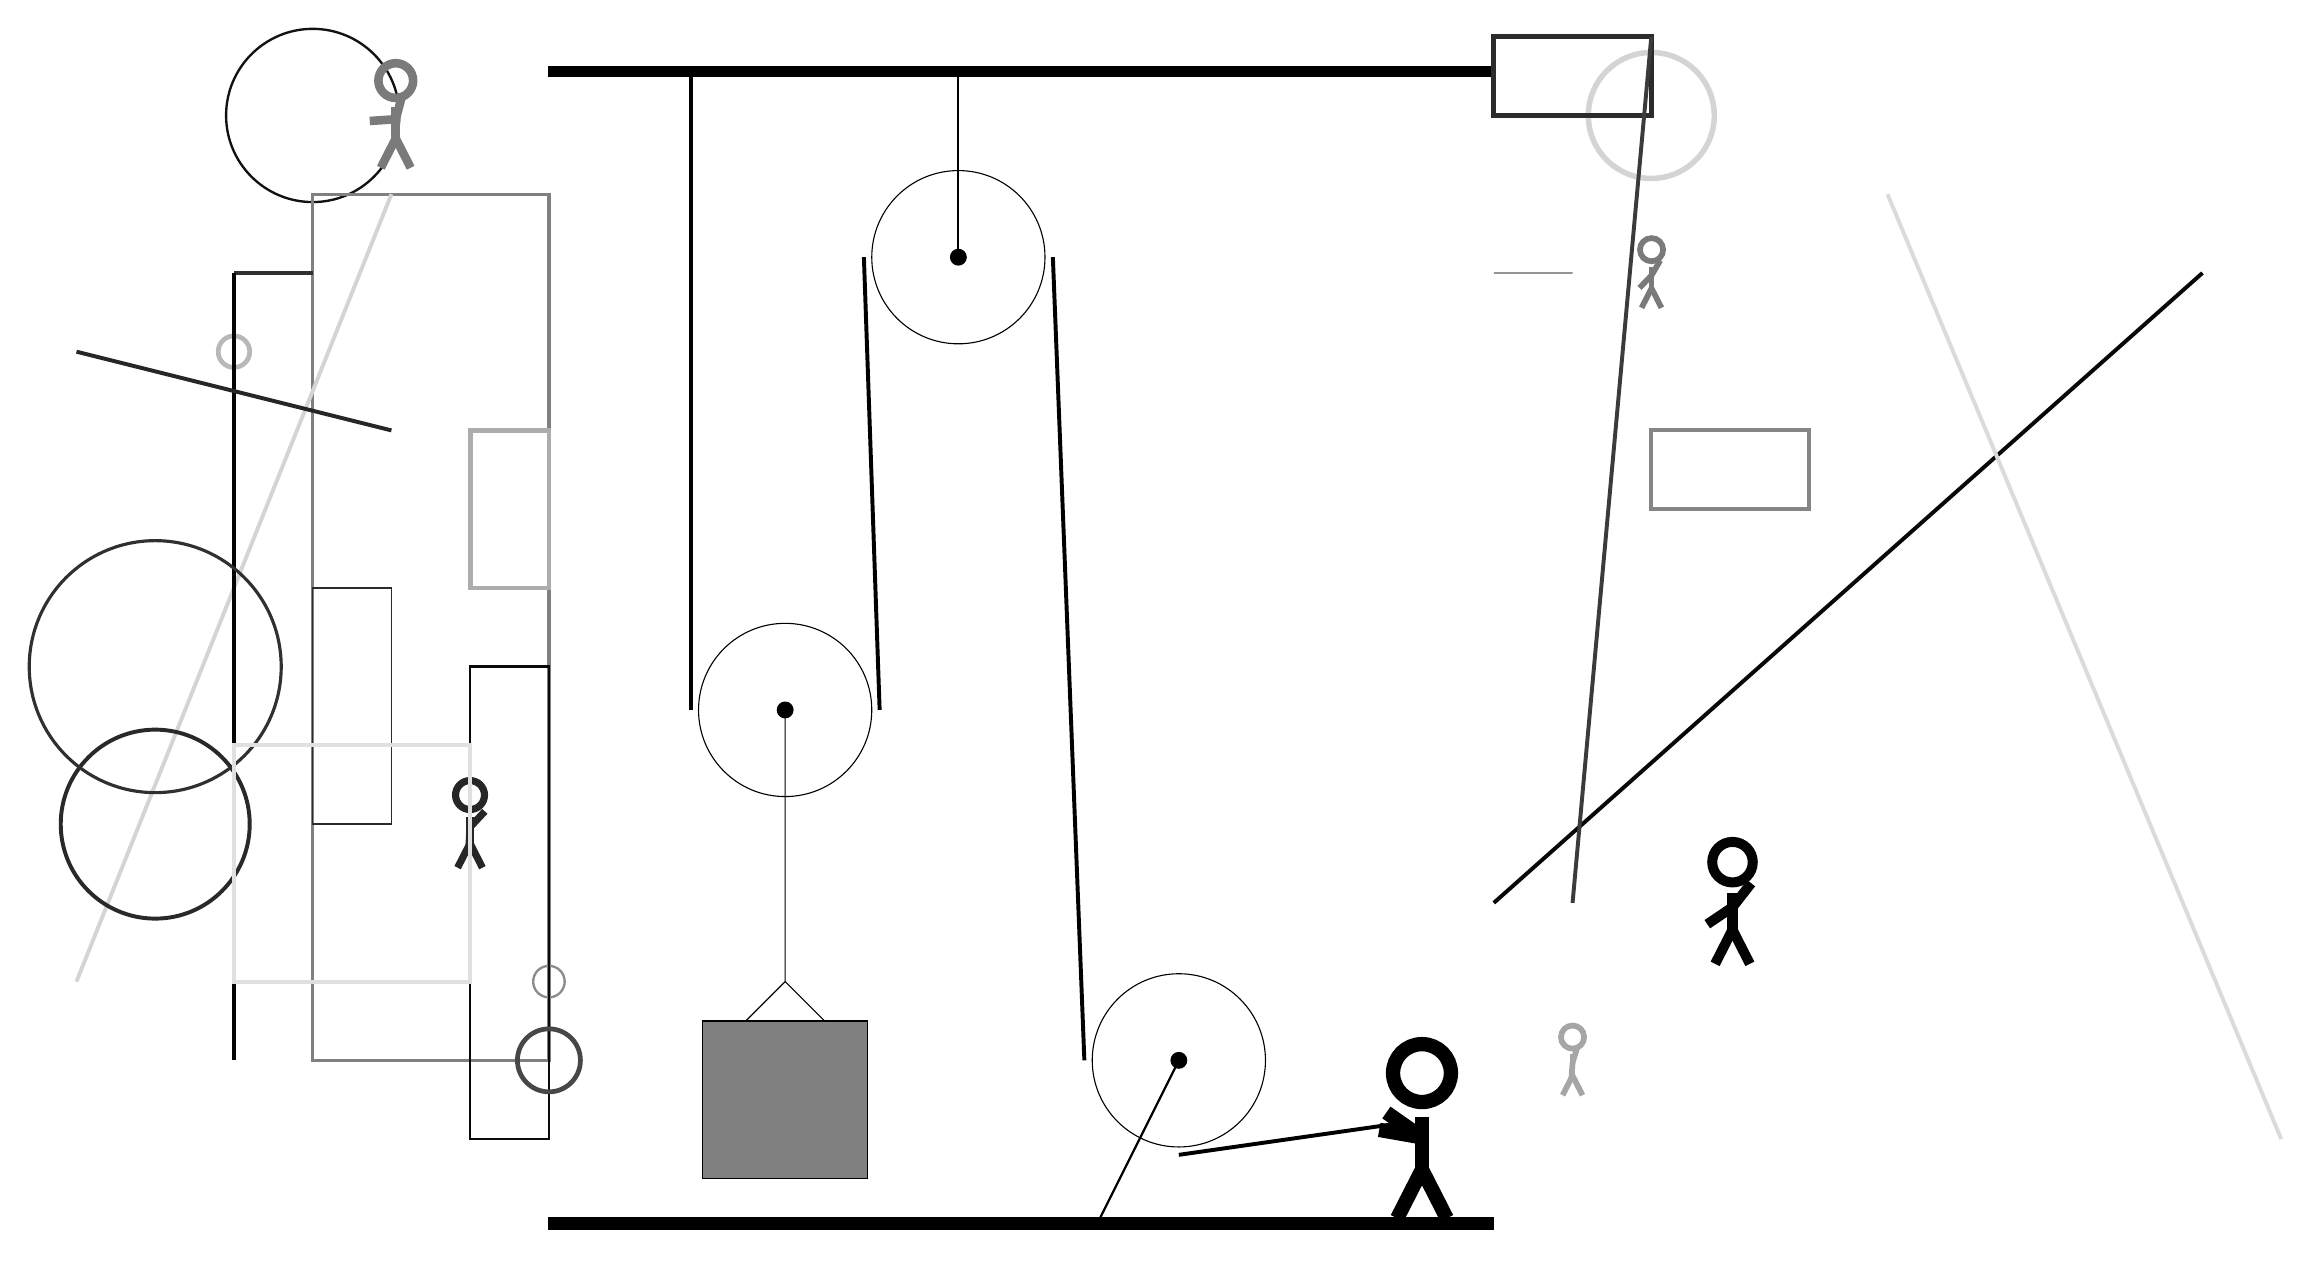
\begin{tikzpicture}
			%%%%% START %%%%%
			
			\draw[fill=black] (-2, 11.5) rectangle (10, 11.625);
			
			\draw (3.2, 9.2) circle (1.1);
			\draw[fill=black] (3.2, 9.2) circle (0.1);
			\draw[thick] (3.2, 9.2) -- (3.2, 11.5);
			
			\draw (6, -1) circle (1.1);
			\draw[fill=black] (6, -1) circle (0.1);
			\draw[thick] (6, -1) -- (5, -3);
			
			\draw (1, 3.45) circle (1.1);
			\draw[fill=black] (1, 3.45) circle (0.1);
			
			\draw (1, 3.45) -- (1, 0.0) -- (0.5, -0.5);
			\draw (1, 0.0) -- (1.5, -0.5);
			\draw[fill=black!50] (-0.05, -0.5) rectangle (2.05, -2.5);
			
			\draw[line width=0.5mm] (-0.2, 11.5) -- (-0.2, 3.45);
			\centerarc[line width=0.5mm](1, 3.45)(180:360:1.2000000000000002);
			\draw[line width=0.5mm](2.2, 3.45) -- (2.0, 9.2);
			\centerarc[line width=0.5mm](3.2, 9.2)(0:180:1.2000000000000002);
			\draw[line width=0.5mm](4.4, 9.2) -- (4.8, -1);
			\centerarc[line width=0.5mm](6, -1)(180:270:1.2000000000000002);
			\draw[line width=0.5mm](6, -2.2) -- (8.8, -1.8);
			
			\node at (9, -1.9) {\Strichmaxerl[10][-35][170]};
			
			\draw [line width=0.3mm, color=black!93](-5, 11) circle (1.1);
			
			\draw [line width=0.6mm, color=black!28](-6, 8) circle (0.2);
			\draw [line width=0.7mm, color=black!17](12, 11) circle (0.8);
			\draw[line width=0.5mm, color=black!48] (12, 7) rectangle (14, 6);
			
			\draw[line width=0.5mm, color=black!97](10, 1) -- (19, 9);
			\draw[line width=0.4mm, color=black!50] (-2, -1) rectangle (-5, 10);
			\draw[line width=0.5mm, color=black!17](-4, 10) -- (-8, 0);
			\draw[line width=0.5mm, color=black!81](-5, 9) -- (-6, 9);
			\draw [line width=0.3mm, color=black!45](-2, 0) circle (0.2);
			\node[line width=0.7mm, color=black!99] at (13, 1) {\Strichmaxerl[7][34][52]};
			
			\draw[line width=0.2mm, color=black!83] (-4, 2) rectangle (-5, 5);
			\node[line width=0.3mm, color=black!52] at (12, 9) {\Strichmaxerl[4][46][60]};
			\draw [line width=0.5mm, color=black!84](-7, 2) circle (1.2);
			
			\draw[line width=0.5mm, color=black!14](15, 10) -- (20, -2);
			\node[line width=0.7mm, color=black!85] at (-3, 2) {\Strichmaxerl[5][87][47]};
			\draw[line width=0.3mm, color=black!96] (-2, 4) rectangle (-3, -2);
			
			\draw[line width=0.6mm, color=black!32] (-3, 5) rectangle (-2, 7);
			\draw[line width=0.6mm, color=black!83] (12, 11) rectangle (10, 12);
			\draw[line width=0.5mm, color=black!77](11, 1) -- (12, 12);
			\draw [line width=0.6mm, color=black!72](-2, -1) circle (0.4);
			\draw[line width=0.3mm, color=black!42] (11, 9) rectangle (10, 9);
			\draw[line width=0.5mm, color=black!99](-6, -1) -- (-6, 9);
			\node[line width=0.7mm, color=black!35] at (11, -1) {\Strichmaxerl[4][86][73]};
			\node[line width=0.5mm, color=black!52] at (-4, 11) {\Strichmaxerl[6][4][75]};
			\draw[line width=0.5mm, color=black!85](-4, 7) -- (-8, 8);
			
			\draw [line width=0.4mm, color=black!81](-7, 4) circle (1.6);
			
			\draw[line width=0.5mm, color=black!12] (-3, 3) rectangle (-6, 0);
			
			\draw[fill=black] (-2, -3) rectangle (10, -3.15);
			
			%%%%% END %%%%%
		\end{tikzpicture}
	\end{figure}	
\end{document}